\section{Project}

\subsection{Hardware}
The following hardware is used:
\begin{itemize}
    \item GTX1060 (6 GB)
\end{itemize}

\subsection{Architecture configuration}
\begin{figure}
    \begin{subfigure}{\textwidth}
        \centering
        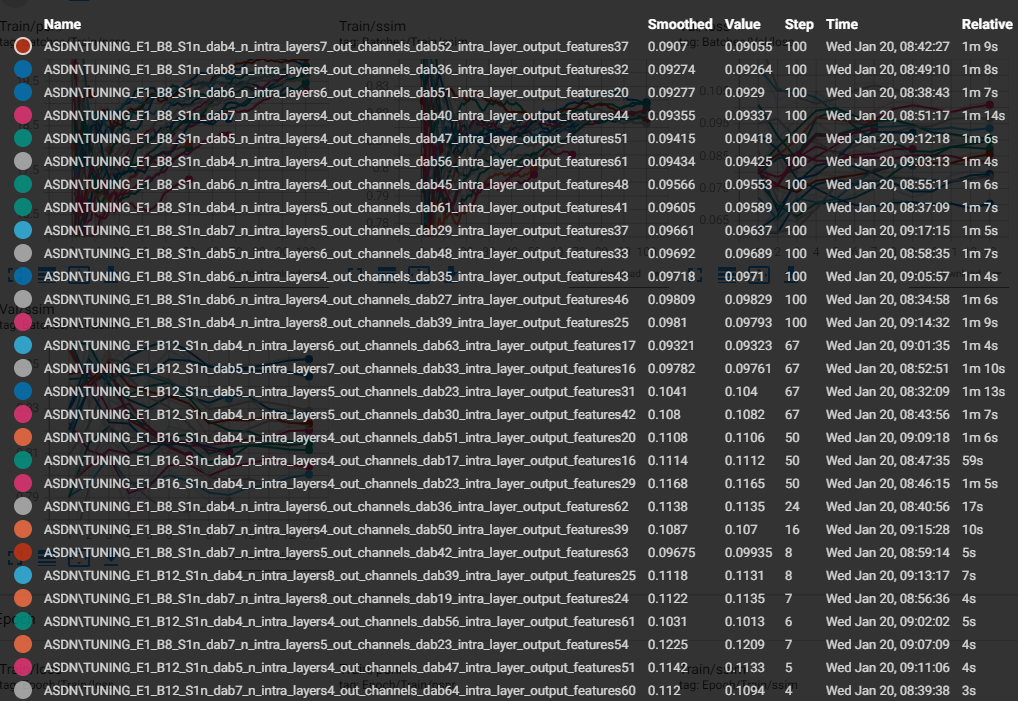
\includegraphics[width=\textwidth, keepaspectratio]{project-tuning-random-configs.png}
        \caption{Training time of different random configurations. There are many other configurations missing due to \textit{out of memory} error.}\label{project:random-configurations}
    \end{subfigure}
    \begin{subfigure}{\textwidth}
        \centering
        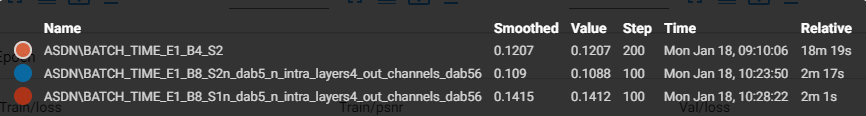
\includegraphics[width=\textwidth, keepaspectratio]{project-tuning-batch-time.png}        
        \caption{Comparison between the training time of 1 epoch of the default configuration, using the trick and not using the trick.}\label{project:batch-time}
    \end{subfigure}

    \caption{Trining time of 1 epoch. The name contains: E is \textit{epoch}, B is \textit{batch size}, S is \textit{save checkpoint} and the network parameters.}    
\end{figure}

\textbf{ASDN} is using a bi-dense connection this means a lot of memory is used for storing intermediate activations as well as gradients: the default configuration, number of dense attention block 16 and number of intra connected layers 8, is not suitable for my computer.

In order to train the default configuration an implementation trick can be used (\textbf{save checkpoint}\footnote{\href{https://pytorch.org/docs/stable/checkpoint.html}{PyTorch checkpoint}}): avoid to store gradient and activations during the forward pass and recompute them during the backward pass; but this increase the training time of a \textbf{single batch} as we can see from \Cref{project:batch-time}

Among many configurations tried [\Cref{project:random-configurations}] the final configuration chosen uses half the parameters with respect to the default configuration:
\begin{tabular}{lc}
    DABs & 8\\
    IDBs & 4\\
    Features DAB & 32 \\
    Features IDB & 32 
\end{tabular}